\documentclass[journal=jpcbfk,manuscript=article,layout=twocolumn]{achemso}
\usepackage{amsmath}
\usepackage{amssymb}
%\usepackage{widetext}
\usepackage{verbatim}
\usepackage{graphicx}
% \usepackage{multicol}
\usepackage[normalem]{ulem} % for strikethrough
\usepackage[obeyFinal]{easy-todo}
\newcommand{\figurewidth}{.48\textwidth}
\renewcommand{\epsilon}{\varepsilon}
\newcommand{\dz}{\,\mathrm{d}z}
\graphicspath{{Figures/}}
\newcommand{\onlinecite}[1]{\hspace{-1 ex} \nocite{#1}\citenum{#1}}
\SectionNumbersOn
%\DeclareUnicodeCharacter{2009}{FIXME}


\author{Hanne S. Antila}
\affiliation{Department of Theory and Bio-Systems, Max Planck Institute of Colloids and Interfaces, 14424 Potsdam, Germany}

\author{Tiago Ferreira}
\affiliation{NMR Group --- Institute for Physics, Martin-Luther University Halle--Wittenberg, 06120 Halle (Saale), Germany}

\author{Matti Javanainen}
\affiliation{Add Matti to author list?}

\author{O. H. Samuli Ollila}
\affiliation{Institute of Biotechnology, University of Helsinki, 00014 Helsinki, Finland}

\author{Markus S. Miettinen}
\affiliation{Department of Theory and Bio-Systems, Max Planck Institute of Colloids and Interfaces, 14424 Potsdam, Germany}
\email{markus.miettinen@mpikg.mpg.de}


\title{Using open data to benchmark internal dynamics of phosphatidylcholine in molecular dynamics simulations}

\begin{document}



\begin{abstract}
Molecular dynamics (MD) simulations are a widely used tool to
    study the atomistic structure and dynamics of biomembranes. It
    remains unknown, however, how well the conformational dynamics
    observed in MD simulations correspond to those occurring in real
    life phospholipids. The accuracy of such time scales in MD can be
    assessed by comparing against the effective correlation times of
    the C-H bonds measured in nuclear magnetic resonance experiments
    (J. Chem. Phys. 142 044905 (2015)).

    Here, we analysed the conformational dynamics of phospholipids as
    produced by several commonly used MD models (force fields). None
    of the tested force fields reproduced all the effective
    correlation times within experimental error, much like they do
    not provide accurate conformational ensemble (J. Phys. Chem. B 119 15075 (2015)). However, the
    dynamics observed in CHARMM36 and Slipids were more realistic
    than those seen in the Amber Lipid14, OPLS-based MacRog, and
    GROMOS-based Berger force fields, which were all characterized by
    unrealistically slow dynamics in the glycerol backbone.
\end{abstract}


\section{Introduction}

Ever since the conception of the Protein Data Bank (PDB) and the NBCI GenBank, the access to open data has shaped the state of the art of research in life sciences.
Not only has the development of new characterisation techniques (such as molecular replacement~\cite{rossmann62} in macromolecular x-ray crystallography and 3D electron microscopy) been aided by the existence of these databases~\cite{burley2018}, but perhaps more importantly they have lead to entirely new ways of doing science in the form of bio- and cheminformatics, enabling data-driven discovery of drugs~\cite{kirchmair08}, materials~\cite{huang2016} as well as identifying~\cite{hobohm1992,levitt2007} and filling~\cite{meszaros2019} gaps in the databanks themselves. All in all, open access to standardised and searchable pools of experimental data, constantly extending owing to a collaborative effort, has enabled scientific progress that is well beyond the resources of one single research group.

%Today these data banks are regarded irreplaceable core resources. The cost of reproducing all the data in PDB has been estimated to be X and destruction of the databank would lead to a near complete halt both academic and commercial research.

Much of the development of the PDB and other biomolecular databanks into the core resources they are today has been fueled by the push from scientific journals and funders towards public availability and conservation of data. In addition to experimental results, these principles have more recently extended to simulation trajectories of biomolecules, leading to databases of dynamic information. Inspired by the success of bio- and cheminformatics, we seek to exploit this and demonstrate, for the first time, the viability of creating new scientific knowledge analysis of pre-existing, open access simulation data. 

More specifically, we will analyze a wide set of publicly available phosphatidylcholine (PC) phospholipid bilayer molecular dynamics (MD) simulation trajectories, produced by using different MD models (force fields). In addition of simulations of one component bilayers under standard conditions, we study trajectories under varying hydration, salt concentration, and cholesterol content. We test whether different force fields reproduce the experimentally observed internal dynamics of PC lipids, and investigate if the dynamics extracted from various models share common features that can be used to draw general conclusions on the system, to suggest future directions for experimental research, and to avoid potential pitfalls in future simulations of bilayers.    

Our choice for the system of interest is inspired by the importance of phospholipids not only as the building blocks of cell membranes but also as emerging candidates for micro- and nanotechnology, such as the use of liposomes as microcapsules in targeted drug delivery~\cite{sercombe15}. These molecules consist of a hydrophilic phosphate head group, which is connected to two hydrophobic fatty acid tails via a glycerol backbone. The ability of lipids to self assemble into bilayer membrane (and other) configurations is a direct consequence of this dual nature. Although biological membranes are complex mixtures of multiple lipid types as well as other molecules, lamellar phospholipid bilayers with one or few lipid types serve as an important model system, that have been successfully used to decipher,  \textit{eg.},  possible molecular mechanisms behind anesthetics~\cite{chau07,XXX}, the effect of cholesterol on membrane structure~\cite{XXX,ferreira13}, and the functioning of membrane proteins~\cite{lindahl08} \todo{add more references}. In particular, MD simulations of these model systems have been widely used~\cite{lyubartsev11,chau07,ferreira13,botan15, ferreira15,miettinen19,XXX} to provide an atomistic view on the biomembranes, and hold vast potential in making further connections between their structure and function.

\begin{comment}
and the conformations adopted by the molecules play a crucial role in determining properties of these lipid assemblies, such as the dipole potential~\cite{Gawrisch92} and the curvature~\cite{XXX}\todo{Markus, any favourite references on curvature?} 

Although biological membranes are complex mixtures of multiple different lipids as well as other molecules, lamellar phospholipid bilayers with one or few lipid types have been successfully used as simplified models systems to decipher,  \textit{eg.},  possible molecular mechanisms behind anesthetics~\cite{chau07,XXX}, the effect of cholesterol on membrane structure~\cite{XXX,ferreira13}, and the functioning of membrane proteins~\cite{lindahl08}. \todo{Markus, do you want to add your favourite topics/references, espc. experimental}. The ability of the simple model membranes to reproduce the biological functioning of headgroup/glycerol structure in cells is backed up by experimental evidence~\cite{gally81}.  In particular, MD simulations of these model systems have been widely used~\cite{lyubartsev11,chau07,ferreira13,botan15, ferreira15,miettinen19,XXX} to provide an atomistic view on the biomembranes, and hold vast potential in making further connections between the structure and the function.

Unfortunately, recent comparison of lipid \mbox{C--H} order parameters from bilayer simulations to nuclear magnetic resonance (NMR) measurements has shown that none of the currently available lipid MD models perfectly reproduces the conformational ensemble sampled by the headgroup~\cite{botan15}. Here, we take a step further and investigate the dynamics of those MD models. 

\end{comment}

The significance for investigating the conformational dynamics of lipids in bilayer simulations is two-fold. Firstly, when exploring static properties of the bilayers, it is crucial to assess how well the simulations have converged. In order to extract reliable statistics, the conformations sampled have to represent the equilibrium distribution with enough transitions between states. Indeed, simulations of a single (1,2-dioleoyl-sn-glycero-3-phosphocholine) DOPC lipid using the CHARMM32b2 force field indicated that the conformations sampled do not replicate the equilibrium distribution even after 500 ns~\cite{vogel12}; also, the C--H bond dynamics of the Berger model was shown~\cite{ferreira15} to be too slow at the glycerol region of 1-palmitoyl-2-oleoylphosphatidylcholine (POPC) compared to correlation times extracted from NMR experiments. 

Secondly, for complete picture of membrane functioning, knowledge on the bilayer dynamics in addition to equilibrium measurements are needed. The ability of the MD model to reproduce the relative abundance of different dynamical processes is crucial for the correct interpretation of pathways leading to, e.g., membrane deformation~\cite{chernomordik08} and lipid-induced conformational~\cite{gibson93,phillips09} changes of membrane proteins. The availability of such model could also greatly guide both the configuration and interpretation of NMR experiments used to extract dynamical information from lipid assemblies. 
\todo{the following paragraph could be merged into methods, opinions?
}
Our analysis of the lipid dynamics is based on two quantities, the spin-lattice relaxation rate $R_{1}$ and the effective correlation time $\tau_\mathrm{e}$, both experimentally available through NMR measurements, and directly calculable from all-atom MD simulations.
Out of the two, the $R_{1}$ rates (or the corresponding $T_{1}$ times) have been traditionally used to assess both the conformational dynamics of lipids in experimental bilayers~\cite{feller02,eldho03,wohlert06,klauda08,leftin11} and the dynamics produced by lipid MD models in bilayer simulations\cite{feller02,wohlert06,klauda08,klauda08II}. However, relying on $R_{1}$ only has several drawbacks~\todo{do all flavors (31P,13C,...) have the same problem?}. It builds on an underlying rotation-diffusion model, its sensitivity is typically limited to C--H bond reorientation with time scales $\sim$1-10 ns, and measurements at several temperatures and magnetic field strengths are required to fully characterize the dynamics. To address these deficiencies, two of us introduced a procedure~\cite{ferreira15} for quantifying the effective C--H correlation times ($\tau_\mathrm{e}$)---a model free quantity that encompasses conformational dynamics with time scales up to hundreds of nanoseconds---from bilayer systems. Most importantly, increasing $\tau_\mathrm{e}$ always signals some type of slowdown in the C--H bond dynamics, making the interpretation less ambiguous than for $R_1$, where slowdown in the dynamics can lead to either an increase or a decrease of $R_{1}$ value~\cite{ferreira15}. 

In summary, this work provides first comprehensive comparison of dynamics of different phosphatidylcholine MD models, where both pure bilayers and the model response to changing conditions and composition is explored. The study is conducted using data-driven exploration of pre-existing, publicly available simulation trajectories to demonstrate the power of open, well documented data in creating new knowledge at a lowered computational cost and high potential for automation.  

---

Q: How is the effective correlation time $\tau_\mathrm e$ related to the autocorrelation of the order parameter $S_\mathrm{CH}$?
After all, $\tau_\mathrm e$ does measure the reorientation of the C--H bond, which is clearly related to how fast the $S_\mathrm{CH}$ is sampled.

A: In a lipid bilayer, the second order rotational correlation function approaches $S^2_\mathrm{CH}$. The speed of this approach tells how fast the C--H bond orientations are sampled. In the relaxation experiment this speed is measured.

In the C--H bond order parameter experiment one measures how much of the second order rotational correlation is left after all the available C--H bond orientations in the bilayer have been sampled.

That is,  $\tau_\mathrm e$ does indeed measure how fast the $S^2_\mathrm{CH}$ is sampled.

If the relaxation is single-exponential, $\tau_\mathrm e$ is the relaxation time of this exponential process. If the relaxation is multi-exponential, $\tau_\mathrm e$ is the weighted mean of the corresponding set of relaxation times.

In the multi-exponential case it is a bit hard to say just based on $\tau_\mathrm e$, how long one needs to sample the $S_\mathrm{CH}$, because this depends also on the above-mentioned weights of the processes.

The main advantage of $\tau_\mathrm e$ is that the larger (smaller) it is, the slower (faster) the process is. The same is not true for R1 or other spin relaxation parameters, because their connection to the molecular dynamics is complicated, and goes through the spectral density, see Eq.~\eqref{eq:R1}.

---

%we intentionally restrict ourselves to re-use existing, publicly available simulation trajectories. This is to demonstrate the power of open, well documented data in creating new knowledge at a lowered cost. The main source of data was the collection of lipid bilayer simulations originating from the NMRlipids project~\cite{botan15,catte16}

%Both the  have been traditionally assessed based on the spin-lattice relaxation rates $R_{1}$ (or the corresponding $T_{1}$ times), available through NMR measurements. At best, the simulation can be combined with the NMR experiments to provide an interpretation of the molecular motion~\cite{pastor88,klauda08,klauda08II}.  


%Here, we use the effective correlation time to present the first comprehensive comparison of dynamics of 1-palmitoyl-2-oleoylphosphatidylcholine (POPC) in different MD models. We not only investigate the pure bilayers in room temperature but also explore the effect of cholesterol content, hydration and monovalent salt to see whether the model dynamics correctly responds to the change in conditions. An MD model fulfilling these requirements can provide a reliable tool to study, e.g., membrane remodeling, or to interpret the experimental spin relaxation rates by connecting them to the underlying dynamical processes. 

%Within this study, we intentionally restrict ourselves to re-use existing, publicly available simulation trajectories. This is to demonstrate the power of open, well documented data in creating new knowledge at a lowered cost. The main source of data was the collection of lipid bilayer simulations originating from the NMRlipids project~\cite{botan15,catte16}. \todo{Start the intro with this, i.e., open data?}


\section{Methods}
\section{Theoretical Background}\label{sec:theory}
$^{13}$C NMR experiments investigating lipid conformational dynamics take advantage of the fact that the relaxation of $^{13}$C magnetization dominantly happens via the dipolar coupling of the carbon with the magnetic moments of the protons bound to it, with the symmetry axis of the interaction aligning with the C--H bond. The spectral density depicting the $^{13}$C relaxation rates (at frequency $\omega$) is expressed as
\begin{equation}
j{(\omega)}=2\int_{0}^{\infty}\cos(\omega\tau)g(\tau)\mathrm d\tau ,
\end{equation}
which is the Fourier transformation of the C--H bond second order autocorrelation function at time $\tau$
\begin{equation}
\label{eq:BCF}
g(\tau)=\langle P_{2}\left(\vec{\mu}(t)\cdot \vec{\mu}(t+\tau)\right)\rangle ,
\end{equation}
where $\vec{\mu}(t)$ is the unit vector in the direction of the C--H bond at time $t$ and $P_{2}$ is the second order Legendre polynomial. The angular brackets depict averaging over time. The autocorrelation function can be expressed as the product of two functions
\begin{equation}
g(\tau)=g_{\mathrm{f}}(\tau)g_{\mathrm{s}}(\tau) ,
\end{equation} 
where $g_{\mathrm{f}}(\tau)$ characterizes fast decays owing to, for example, the molecular  rotations, and $g_{\mathrm{s}}(\tau)$ describes slow decays that originate from, e.g., the lipid diffusion. The two components, along with the oscillation due to magic angle spinning at the $\sim$kHz region, are depicted in Fig.~\ref{fig:schem_teff}. Correlation time of 4.2 ms has been estimated for multilamellar POPC samples at 300 K for the slow modes, whereas  in liquid crystalline lipid bilayers the faster $g_{\mathrm{f}}(\tau)$ decays to a plateau value $S^{2}_{\rm{CH}}$ within a few hundred nanoseconds~\cite{ferreira15}. The C--H bond order parameters
\begin{equation}
\label{eq:OP}
S_{\rm{CH}}=\frac{1}{2}\langle 3\cos^{2}\theta-1\rangle ,
\end{equation}
where $\theta$ is the angle between the bond and the bilayer normal, are measured in NMR experiments from this plateau. As $S_{\rm{CH}}$ describes the conformational ensemble of the molecule, the fast-decaying component of the rotational correlation function intuitively depicts the time needed to sample these conformations. The characteristic time can be quantified via the effective correlation time
\begin{equation}
\label{eq:teff}
\tau_\mathrm{e}=\int_{0}^{\infty}\frac{g_{\mathrm{f}}(\tau)-S^{2}_{\rm{CH}}}{1-S^2_{\mathrm{CH}}}\mathrm d\tau.
\end{equation}
The integrand can be viewed as a reduced and normalized correlation function
\begin{equation}
\label{eq:nBCF}
g'_{\mathrm{f}}(\tau)=\frac{g_{\mathrm{f}}(\tau)-S^{2}_{\rm{CH}}}{1-S^2_{\mathrm{CH}}}.
\end{equation}
That is, $\tau_\mathrm e$ is defined as the area under $g'_{\mathrm{f}}(\tau)$, as
graphically depicted in Fig.~\ref{fig:schem_teff}b.
\todo{Maybe also add 1C that explicitly shows $g'_{\mathrm{f}}$?}
It is easily seen that in the presence of more long-lived correlations $\tau_\mathrm{e}$ grows, signaling that more time is needed for full conformational sampling.  

\begin{figure}[t]
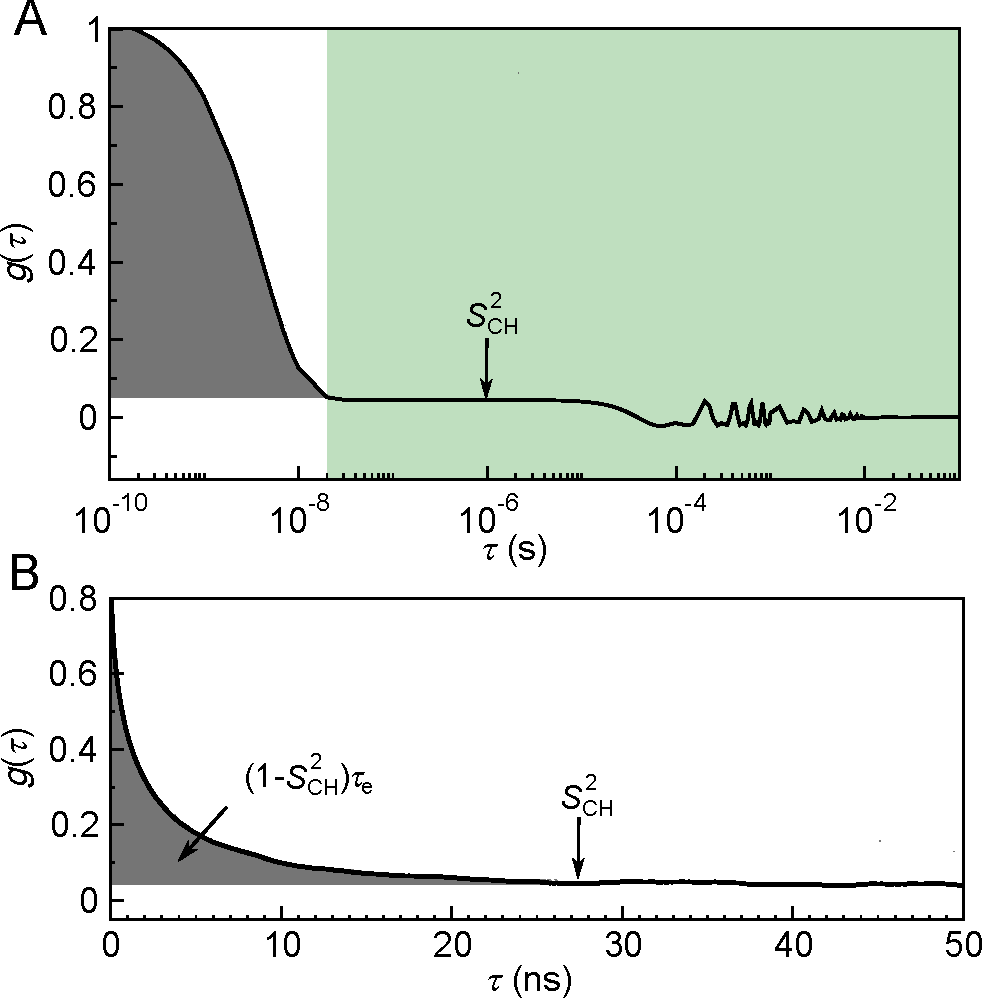
\includegraphics[scale=0.45]{gfun_wg.pdf} 
\caption{The autocorrelation function $g(\tau)$ a) The fast mode (white background) and the slow mode (shaded green) of the correlation function along with the oscillation owing to magic angle spinning. The fast mode decays to a plateau quantifying the $S_{\mathrm{CH}}$ while the slow mode gives the final descent to zero. b) Illustration of typical C--H bond autocorrelation function obtained from a MD simulation. The gray area under the curve gives a means of quantifying the $\tau_\mathrm{e}$. }
\label{fig:schem_teff}

\end{figure} 

The bond correlation functions are readily available from MD simulations. In addition to extracting $\tau_\mathrm{e}$ directly by integrating the area, fitting a set of $N$ exponentials, each with their own correlation times $\tau_{i}$ to the normalized correlation function 
\begin{equation}
g'_\mathrm{MD}(t)=\sum_{i=1}^{N}\alpha_{i}e^{-t/\tau_{i}}
\end{equation}
provides an alternative way of quantifying $\tau_\mathrm{e}$ 
\begin{equation}
\tau_\mathrm{e}=\sum_{i=1}^{N}\alpha_{i}\tau_{i} .
\end{equation}
When the simulation trajectory is not long enough for the correlation function to reach the plateau, integrating the area gives a lower bound estimate for $\tau_\mathrm{e}$, while the latter method includes also (some) contribution from the longer-time components via the fitting process.
However, in practice the fit is often highly unreliable in terms of depicting the long tails of the correlation function, and in this work we choose to quantify $\tau_\mathrm{e}$ using the area.

The spin-lattice relaxation rate $R_1$ defines the time-scale on which $^{13}$C longitudal magnetization equilibrates. It is defined as  
\begin{equation}
\label{eq:R1}
\begin{aligned}
R_{1}=\frac{d^2_{\mathrm{CH}}N_{\mathrm{H}}}{20}\left[j(\omega_{\mathrm{H}}-\omega_{\mathrm{C}})\right. \\
\left.+3j(\omega_{\mathrm{C}})+6j(\omega_{\mathrm{H}}+\omega_{\mathrm{C}})\right] ,
\end{aligned}
\end{equation}
where $N_{\mathrm{H}}$ is the number of bound hydrogens, $\omega_{\mathrm{H}}$ and $\omega_{\mathrm{C}}$ are the Larmor frequencies for $^{1}$H and $^{13}$C, and $d_{\mathrm{CH}}$ is the rigid dipolar coupling constant. For the methylene bond, $d_{\mathrm{CH}}/2\pi$ approximately equals to -22~kHz.


The dependency of $R_{1}$ on the spectral densities $j$ at the Larmor frequencies means that the $R_{1}$ value depicts the relative amounts of relaxation processes with time-scales near the inverses of the Larmor frequencies. Since the Larmor frequencies depend on the field strength used in the NMR measurements, this typically makes $R_{1}$ sensitive to $\sim$1--10~ns time-scales. Importantly, a change in $R_{1}$ thus indicates a difference in the relative amounts of processes within the detection window, and therefore does not give information on the modulation of the total sampling rate.  


\begin{comment}
 The dipolar coupling constant $d_{\mathrm{CH}}$ is defined as

\begin{equation}
d_{\mathrm{CH}}=\frac{\hslash\gamma_{\mathrm{H}}\gamma_{\mathrm{C}}\mu_{0}}{4\pi\langle r^{3}_{\mathrm{CH}} \rangle} ,
\end{equation}

where $\hslash$ is the reduced Planck constant, $\gamma_{\mathrm{C}}$ and $\gamma_{\mathrm{H}}$ are the gyromagnetic constants for $^{1}H$ and $^{13}C$, $\mu_{0}$ is the vacuum permeability, and $\langle r^{3}_{\mathrm{CH}}\rangle$ denotes the average cubic length of the C-H bond.
\end{comment}

\subsection{Data aquisition and analysis}

The simulation trajectories used in this work were collected from the Zenodo repository (\url{zenodo.org}) with majority of the data originating from the NMRlipids project~\cite{botan15,catte16} (\url{nmrlipids.blogspot.fi}). A list of the simulations, as well as the references to the data files are presented in Table~\ref{tab:standr} for trajectories near room temperature and in full hydration, Table~\ref{tab:chol} for simulations including cholesterol, Table~\ref{tab:hydr} for data under varying hydration, and Table~\ref{tab:salt} for simulations in increasing NaCl concentration. Additional computational details of each of the simulations are available at the referred Zenodo entry. All the experimental quantities were collected from the literature \todo{Except are they, or mostly from Tiago and re-analysed from raw data?} sources referred at the respective figures\todo{How to refer to experimental data from Tiago?}.   

\begin{table}[t!]
\caption{Analyzed simulations of POPC bilayers under full hydration. The column labeled "files" lists the citation numbers that contain links to the downloadable simulation files. Number of lipids and number of water molecules are denoted with N$_{{\rm l}}$ and N$_{{\rm w}}$, respectively, temperatures (T) are given in Kelvins and t$_{{\rm anal}}$ is the length of the trajectory used for analysis.}
\resizebox{8.7cm}{!} {
\begin{tabular}{llrrrrc}
%\hline
force field  & lipid & N$_{{\rm l}}$  & N$_{{\rm w}}$  & T (K)  & t$_{{\rm anal}}$ (ns) & files \tabularnewline
\hline 
Berger-POPC-07~\cite{ollila07a}  & POPC & 128 & 7290 & 298 & 50  & {[}\!\!\citenum{bergerFILESpopc}{]} \tabularnewline
CHARMM36~\cite{klauda10} & POPC  & 128 & 5120 & 303 & 140 & {[}\!\!\citenum{charmm36files}{]} \tabularnewline
CHARMM36~\cite{klauda10} & POPC & 34 & 1020 & 300 & 140 & {[}\!\!\citenum{charmm36filesHA}{]}\tabularnewline
MacRog~\cite{kulig15}  & POPC  & 128  & 6400 & 310 & 200  & {[}\!\!\citenum{macrogCHOLfiles}{]}\tabularnewline
Lipid14 \cite{dickson14}  & POPC  & 72 & 2234 & 303 & 50 & {[}\!\!\citenum{lipid14files}{]}\tabularnewline
Slipids \cite{jambeck12b}  & POPC  & 200 & 9000 & 310 & 500  & {[}\!\!\citenum{slipidsFILESpopcchol}{]}\tabularnewline
ECC \cite{melcr18}  & POPC  & 128 & 6400 & 300 & 300  & {[}\!\!\citenum{eccFILESpopc}{]}\tabularnewline
\end{tabular}}
\label{tab:standr}
\end{table}

\begin{table}[t!]
\caption{Simulation data for cholesterol-containing POPC bilayers. Number of cholesterols is given by N$_{{\rm chol}}$ while C$_{{\rm chol}}$ denotes the percentage of cholesterol from all the lipids. Rest of the labels are as in Table~\ref{tab:standr}.}
\resizebox{8.7cm}{!} {
\begin{tabular}{llrrrrrrc}
%\hline
force field  & lipid  & N$_{{\rm l}}$  & N$_{{\rm chol}}$  & C$_{{\rm chol}}$  & N$_{{\rm w}}$  & T (K)  & t$_{{\rm anal}}$ (ns) & files \tabularnewline
\hline 
Berger-POPC-07~\cite{ollila07a} & POPC  & 128  & 0  & 0\%  & 7290  & 298  & 50 & {[}\!\!\citenum{bergerFILESpopc}{]} \tabularnewline
/H\"{o}ltje-CHOL-13~\cite{holtje01,ferreira13}  & POPC  & 64  & 64  & 50\%  & 10314  & 298  & 60  & {[}\!\!\citenum{bergerFILESpopc50chol}{]} \tabularnewline
CHARMM36\cite{klauda10,lim12}  & POPC  & 128 & 0 & 0\%  & 5120  & 303  & 140  & {[}\!\!\citenum{charmm36files}{]} \tabularnewline
 & POPC  & 80  & 80  & 50\%  & 4496  & 303  & 200  & {[}\!\!\citenum{charmm36files50perCHOL}{]} \tabularnewline
MacRog\cite{kulig15}  & POPC  & 128  & 0  & 0\%  & 6400  & 310  & 200  & {[}\!\!\citenum{macrogCHOLfiles}{]} \tabularnewline
 & POPC  & 64  & 64  & 50\%  & 6400  & 310  & 200  & {[}\!\!\citenum{macrogCHOLfiles}{]} \tabularnewline
Slipids \cite{jambeck12b,jambeck13chol} & POPC  & 200  & 0 & 0\% & 9000 & 310 & 500  & {[}\!\!\citenum{slipidsFILESpopcchol}{]} \tabularnewline
 & POPC & 200 & 200 & 50\% & 18000 & 310 & 500 & {[}\!\!\citenum{slipidsFILESpopcchol}{]}\tabularnewline
\end{tabular}}
\label{tab:chol}
\end{table}

\begin{table}[h!]
\caption{Simulation data for bilayers under varying hydration level. The water to lipid ratio is denoted as W/L, and other labels are as in Table~\ref{tab:standr}.}
\resizebox{8.7cm}{!} {
\begin{tabular}{llrrrrrc}
%\hline
force field  & lipid  & W/L  & N$_{{\rm l}}$  & N$_{{\rm w}}$  & T (K)  & t$_{{\rm anal}}$ (ns) & files \tabularnewline
\hline 
Berger-POPC-07~\cite{ollila07a}  & POPC  & 57  & 128  & 7290  & 298  & 50 & {[}\!\!\citenum{bergerFILESpopc}{]} \tabularnewline
 & POPC  & 7  & 128  & 896  & 298  & 60  & {[}\!\!\citenum{bergerDEHYDfiles}{]} \tabularnewline
 Berger-DLPC-13~\cite{kanduc13} & DLPC  & 24  & 72  & 1728  & 300  & 80  & {[}\!\!\citenum{bergerFILESdlpc24}{]} \tabularnewline
 & DLPC  & 16  & 72  & 1152  & 300  & 80  & {[}\!\!\citenum{bergerFILESdlpc16}{]} \tabularnewline
 & DLPC  & 12  & 72  & 864  & 300  & 80  & {[}\!\!\citenum{bergerFILESdlpc12}{]} \tabularnewline
 & DLPC  & 4  & 72  & 288  & 300  & 80  & {[}\!\!\citenum{bergerFILESdlpc4}{]} \tabularnewline
CHARMM36\cite{klauda10}  & POPC  & 40  & 128  & 5120  & 303  & 140 & {[}\!\!\citenum{charmm36files}{]} \tabularnewline
 & POPC  & 15  & 72  & 1080  & 303  & 20  & {[}\!\!\citenum{charmm36files15wPERl}{]} \tabularnewline
 & POPC  & 7  & 72  & 504  & 303  & 20  & {[}\!\!\citenum{charmm36files7wPERl}{]} \tabularnewline
MacRog\cite{kulig15}  & POPC  & 50  & 288  & 14400  & 310  & 40  & {[}\!\!\citenum{macrogdehydFILES}{]} \tabularnewline
 & POPC  & 15  & 288  & 4320  & 310  & 100 & {[}\!\!\citenum{macrogdehydFILES}{]} \tabularnewline
 & POPC  & 10  & 288  & 2880  & 310  & 100  & {[}\!\!\citenum{macrogdehydFILES}{]} \tabularnewline
\end{tabular}}
\label{tab:hydr}
\end{table}

%\begin{multicols}{2}
%\twocolumn
\begin{table*}[t!]
\caption{Simulation data for bilayers under varying concentration of NaCl. Number of Na$^+$ and Cl$^-$ ions are denoted by N$_{{\rm Na}}$ and N$_{{\rm Cl}}$ while {[}salt{]} gives the NaCl concentration calculated as {[}salt{]} =N$_{{\rm Na}}${[}water{]}/N$_{{\rm w}}$, where {[}water{]} = 55.5 M. Other labels are as in Table~\ref{tab:standr}.}
\resizebox{16cm}{!} {
\begin{tabular}{llrrrrrrrc}
%\hline
% some footnotes are not visible in typeset-MS (pdf)
force field (lipid, ion) & lipid  & {[}salt{]} mM  & N$_{{\rm l}}$  & N$_{{\rm w}}$  & N$_{{\rm Na}}$  & N$_{{\rm Cl}}$  & T (K)  & t$_{{\rm anal}}$ (ns)  & files\tabularnewline
\hline 
CHARMM36\cite{klauda10}  & POPC  & 0 & 128  & 5120  & 0 & 0 & 303 & 140 & {[}\!\!\citenum{charmm36files}{]}\tabularnewline
CHARMM36\cite{klauda10}, CHARMM36\cite{venable13}  & POPC  & 350 & 72  & 2085  & 13  & 13  & 303  & 80  & {[}\!\!\citenum{charmmPOPC350mMNaClfiles}{]} \tabularnewline
CHARMM36\cite{klauda10}, CHARMM36\cite{venable13}  & POPC  & 690 & 72  & 2085  & 26  & 26  & 303  & 73 & {[}\!\!\citenum{charmmPOPC690mMNaClfiles}{]} \tabularnewline
CHARMM36\cite{klauda10}, CHARMM36\cite{venable13}  & POPC  & 950 & 72  & 2168  & 37  & 37  & 303  & 60  & {[}\!\!\citenum{charmmPOPC950mMNaClfiles}{]} \tabularnewline
\hline 
MacRog\cite{kulig15}  & POPC  & 0  & 128  & 6400  & 0 & 0 & 310 & 400 & {[}\!\!\citenum{macrogCHOLfiles}{]}\tabularnewline
MacRog\cite{kulig15}, OPLS\cite{aqvist90}  & POPC  & 100 & 288  & 14554  & 27  & 27  & 310  & 90 & {[}\!\!\citenum{macrogIONfiles}{]} \tabularnewline
MacRog\cite{kulig15}, OPLS\cite{aqvist90}  & POPC  & 210  & 288  & 14500  & 54  & 54  & 310  & 90  & {[}\!\!\citenum{macrogIONfiles}{]} \tabularnewline
MacRog\cite{kulig15}, OPLS\cite{aqvist90}  & POPC  & 310 & 288  & 14446  & 81  & 81  & 310  & 80  & {[}\!\!\citenum{macrogIONfiles}{]} \tabularnewline
MacRog\cite{kulig15}, OPLS\cite{aqvist90}  & POPC  & 420 & 288  & 14392  & 108  & 108  & 310  & 90 & {[}\!\!\citenum{macrogIONfiles}{]} \tabularnewline
\hline 
Slipids \cite{jambeck12b}  & POPC  & 0 & 200  & 9000 & 0 & 0 & 310 & 500 & {[}\!\!\citenum{slipidsFILESpopcchol}{]}\tabularnewline
Slipids\cite{jambeck12b}, AMBER\cite{smith94}  & POPC  & 130 & 200  & 9000  & 21  & 21  & 310  & 100 & {[}\!\!\citenum{slipidsFILESpopc130mMnaclSD}{]} \tabularnewline
Slipids\cite{jambeck12b}, AMBER\cite{smith94} & POPC & 1.0 & 200 & 900 & 162 & 162 & 310 & 200 & {[}\!\!\citenum{slipidsFILESpopc1MnaclSD}{]}\tabularnewline
\end{tabular}}
\label{tab:salt}
\end{table*}
%\onecolumn
%\end{multicols}

The simulational data were analysed using in-house scripts. These are available on GitHub \cite{citehere} along with a Python notebook outlining an example analysis run.
After downloading the necessary files from Zenodo, the trajectory was processed with Gromacs \texttt{gmx trjconv} to make the molecules whole.
The C--H bond order parameters  $S_\mathrm{CH}$, see Eq.~\eqref{eq:OP}, were then calculated with the \texttt{calcOrderParameters.py}\cite{citegithubhere} script that uses the MDanalysis\cite{XXX} Python library.
%
The \mbox{C--H} bond correlation functions
$g(\tau)$, see Eq.~\eqref{eq:BCF},
were calculated with Gromacs5.1.4\cite{XXX} \texttt{gmx rotacf};
note that on these (fast) time scales $g = g_\mathrm{s} g_\mathrm{f}= g_\mathrm{f}$.
%
To obtain the $g'_\mathrm f$,
the $S_\mathrm{CH}$ were used to
normalize the $g_\mathrm f$ following Eq.~\eqref{eq:nBCF}.
%
Finally, the effective correlation times $\tau_\mathrm e$ were calculated by integrating, see Eq.~\eqref{eq:teff},
$g'_\mathrm f(\tau)$ over time from $\tau=0$ until $\tau = t_0$.
Here
$t_0 = \min
	\{
	t\,|\,g'(t)=0
	\}
$,
that is, $t_\mathrm 0$ is the first time point at which $g'_\mathrm f$ reached zero.
%
If $g'_\mathrm f$ did not reach zero within 
$t_\mathrm{anal}/2$, the 
$\tau_\mathrm e$ was not determined,
but we report only its upper and lower error estimates.

To estimate the error on $\tau_\mathrm e$, we first estimate the error on $g'_\mathrm f(\tau)$.
%
%At a given timepoint $\tau$,
There are two sources of error, $g_{\mathrm{f}}(\tau)$ and $S^2_\mathrm{CH}$.
%
Performing linear error propagation on Eq.~\eqref{eq:nBCF} gives
\begin{align}
\begin{split}
\label{eq:error}
\Delta g'_{\mathrm{f}}(\tau)
%=
%\frac{\mathrm d g'_\mathrm{f}(\tau)}{\mathrm d g_{\mathrm{f}}(\tau)}\Delta g_{\mathrm{f}}(\tau)
%+
%\frac{\mathrm d g'_\mathrm{f}(\tau)}{\mathrm dS_\mathrm{CH}}\Delta S_\mathrm{CH}
=
&\left|
	\frac{1}{1-S^2_\mathrm{CH}}
\right|
\Delta g_{\mathrm{f}}(\tau)\\
&+\\
&\left|
	\frac{2\left(g_\mathrm{f}(\tau)-1\right)S_\mathrm{CH}}{\left(1-S^2_\mathrm{CH}\right)^2}
\right|
\Delta S_\mathrm{CH}.
\end{split}
\end{align}
Here the $\Delta S_\mathrm{CH}$ was determined as in the NMR\-lipids Project:
the standard error of the mean of the $S_\mathrm{CH}$ of all the individual lipids~\cite{botan15}.
%
Similarly, we determined the error on $g_{\mathrm{f}}(\tau)$
by first determining an individual correlation function $g^m_{\mathrm{f}}(\tau)$ for each lipid $m$
over the whole trajectory, and then obtaining the error estimate
$\Delta g_{\mathrm{f}}(\tau)$
as the standard error of the mean over the lipids.
%
Importantly, this gives an error estimate at each time point $\tau$.

To obtain the lower error estimate on $\tau_\mathrm e$, we integrate the function
$g'_{\mathrm{f}}(\tau) - \Delta g'_{\mathrm{f}}(\tau)$ over time from $\tau=0$ until $\tau=t_\mathrm l$.
Here
\begin{equation}
t_\mathrm l= \min
\left\{
	\left\{
		t\,|\,g'_{\mathrm{f}}(t) - \Delta g'_{\mathrm{f}}(t) = 0
	\right\},
	\frac{t_\mathrm{anal}}{2}
\right\}.
\end{equation}
That is,
$t_\mathrm l$ is
the first time point at which the lower error estimate of $g'_\mathrm f$ reached zero;
or $t_\mathrm l=t_\mathrm{anal}/2$, if zero was not reached by that point.
%This is the one sigma error.

To obtain the upper error estimate on $\tau_\mathrm e$, we first integrate the function
$g'_{\mathrm{f}}(\tau) + \Delta g'_{\mathrm{f}}(\tau)$ over time from $\tau=0$ until
$
t_\mathrm u= \min
\left\{
	t_0,
	{t_\mathrm{anal}}/{2}
\right\}.
$
Note, however,
that this is not yet sufficient, because there could be slow processes that our simulation was not
able to see. Although these would contribute to $\tau_\mathrm e$ with a low weight,
their contribution over long times could still add up to a sizable effect on $\tau_\mathrm e$.
%
That said, it seems feasible to assume (see Fig. \ref{fig:schem_teff}A) that there are no longer-time contributions
to $g_\mathrm f$ than something that decays with a time constant of $10^{-6}$~s.
%
We use this as our worst case estimate to assess the upper error on $\tau_\mathrm e$, and
%
assume that all the decay from the time point
$
t_\mathrm u= \min
\left\{
	t_0,
	{t_\mathrm{anal}}/{2}
\right\}
$
onwards comes solely from this slowest process.
%
The additional contribution to the upper error for $\tau_\mathrm e$ then reads
$
\Delta g'_\mathrm f(t_\mathrm u) \times \left(\exp(-t_\mathrm u / 10^{-6}\,\mathrm s) - \exp(-1)\right) \times 10^{-6}\,\mathrm s.
$

The $R_{1}$ were first calculated separately for each lipid in the system using Eq.~\eqref{eq:R1} and then averaging over the lipids. The standard error of mean was used to estimate the uncertainty in $R_{1}$. The spectral densities for Eq.~\eqref{eq:R1} were obtained by fitting a sum of 71 exponentials, with logarithmically spaced time-scales $\tau_{i}$ ranging from 0.1 ns to 1 $\mu$s, to the normalized correlation functions $g'^m_{\mathrm{f}}(t)=\sum_{i=1}^{N}\alpha_{i}e^{-t/\tau_{i}}$ and then calculating the spectral density based of the Fourier transformation\cite{ferreira15}
\begin{equation}
j^m{(\omega)}=2(1-S_\mathrm{CH})\sum_{i=1}^{N}\alpha_{i}\frac{\tau_{i}}{1+\omega\tau_{i}} .
\end{equation}

\todo{Discuss the possibility of skewed error distributions?}

\section{Results and Discussion}
\subsection*{Effective correlation times at standard conditions.}
The upper panels of Fig.~\ref{fig:teff_R1} compare the $\tau_\mathrm{e}$ obtained for fully hydrated POPC bilayers in experiments (black) and in six different MD force fields (color).

Qualitatively, every force field captures the general shape of the $\tau_\mathrm{e}$ profile: Dynamics slows down towards the glycerol backbone in both the headgroup and in the tails. Quantitatively, the $\tau_\mathrm{e}$ in the membrane core are reproduced rather well, but at the water-facing interface MD has a tendency towards slower dynamics than what was experimentally observed.
CHARMM36 and Slipids have the best overall performance---although Slipids exhibits a qualitatively wrong, decreasing, trend from $\mathrm g_{3}$ to $\mathrm g_{1}$. \todo{Not extremely clear, though; would be good to know the errors to make this claim.}

The slowness of MD around the glycerol backbone is consistent with previous results for the Berger model~\cite{ferreira15}. It also agrees with the insufficient conformational sampling of glycerol backbone torsions observed in 500-ns-long CHARMMc32b2~\cite{schlenkrich96,feller00} simulations of a DOPC lipid~\cite{vogel12}. % The first carbon of the palmitoyl tail is the only location where some force fields have a tendency to underestimate $\tau_{\mathrm{eff}}$. 

We emphasize that the simulation data in Fig.~\ref{fig:teff_R1} give a \emph{lower} limit of $\tau_\mathrm{e}$, as discussed in Theoretical Background (Sec.~\ref{sec:theory}). The $\tau_\mathrm{e}$ values could increase further if the trajectories were extended, and thus the true overestimation could be more severe than what was seen here.

It is also worth noting that the temperature for simulation data varied across the models, but in no simulation was it lower than in the experiment. %As one would expect $\tau_\mathrm{e}$ to decrease with increasing temperature, the slow dynamics observed in some force fields do not occur because of the temperature difference.
Also, the data are practically identical for the two CHARMM36 simulations that differ in system size and temperature, which indicates that small variations in either do not considerably affect the $\tau_\mathrm{e}$.

\begin{figure}[!ht]
\centering
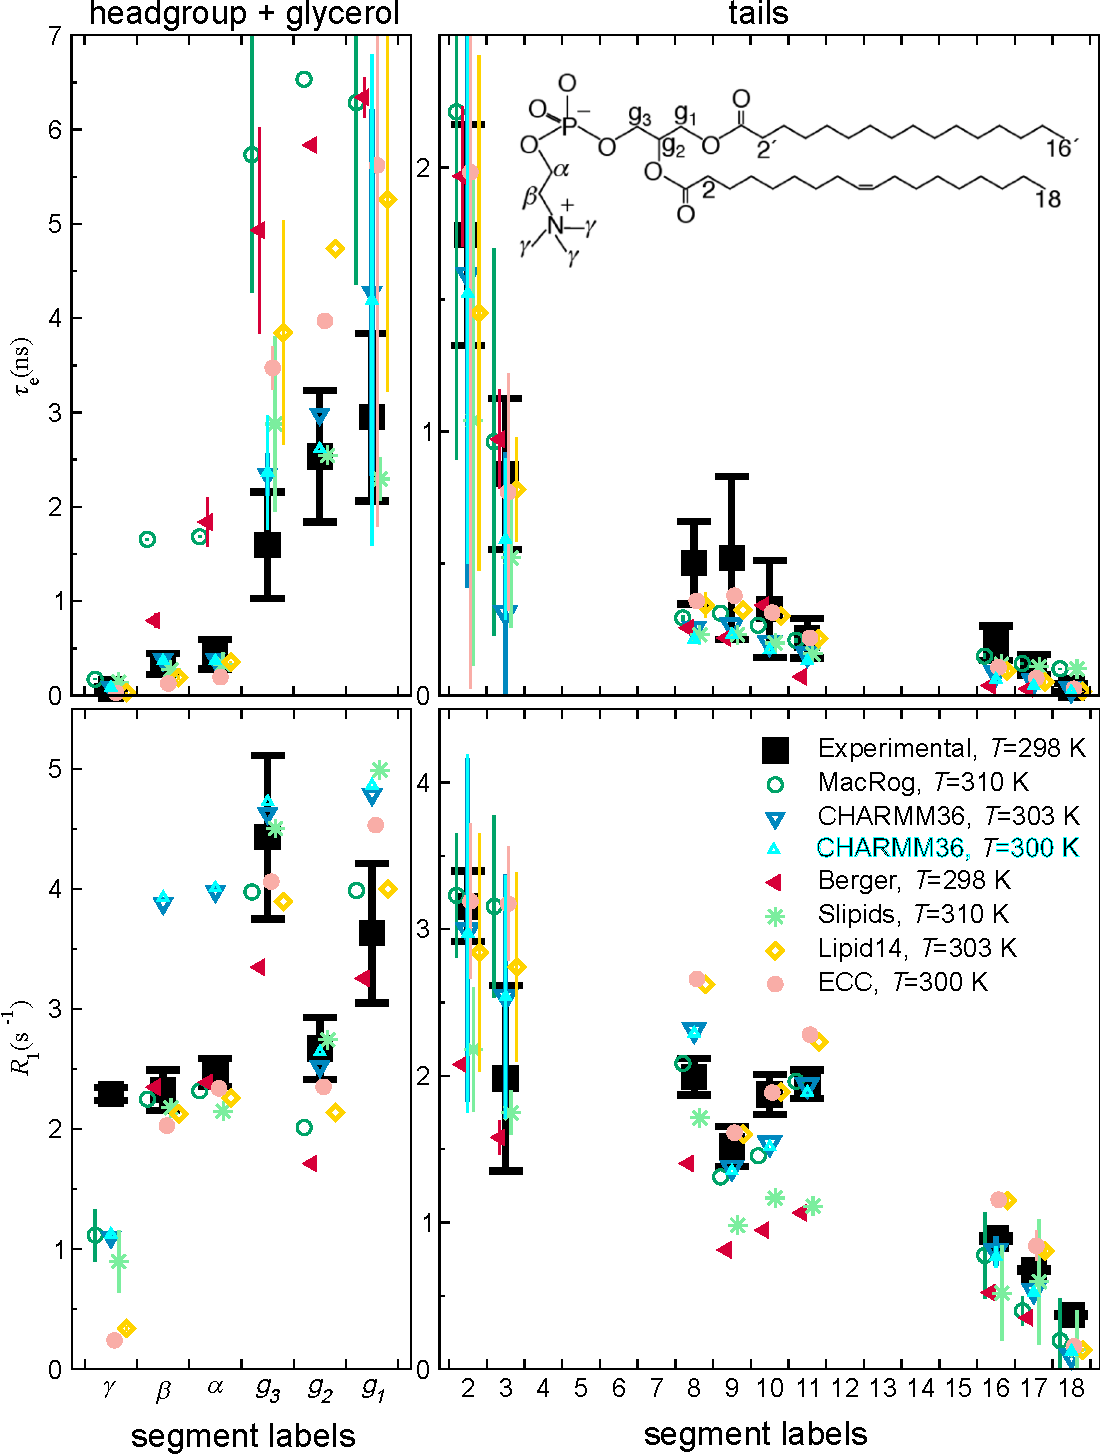
\includegraphics[width=0.9\columnwidth]{normalcond.pdf}
\caption{Effective correlation times ($\tau_\mathrm{e}$, upper panels) and $R_{1}$ rates (lower panels) in experiments (black) and MD simulations (colored) of POPC bilayers in $L_{\alpha}$ phase under full hydration.
Inset shows the POPC structure and segment labelling.
The data for  segments 8--11 is from the sn-2 (oleoyl) chain, whereas non-resolved contributions from both tails are included for segments 2--3 (2'--3' in the sn-1 chain) and 16--18 (14'--16').
Simulation data is shown only for the segments for which there was experimental data.
The methyl segments ($\gamma$, C18, and C16') in Berger are left out, because for a united atom model the hydrogens are constructed, post-simulation, from the heavy atom locations, and the protonation algorithm does not preserve the methyl C--H bond dynamics.
Error bars for the experimental values reflect error estimate of {\color{red}XXX}, whereas the 
bars for simulated data points give the minimum and maximum value observed at each segment while the symbol denotes the average. %For the simulated data this includes contributions from both chains for carbon labels 2--3 and 16--18, in line with the experimental data. 
Table~\ref{tab:standr} provides further simulation details.
}
\label{fig:teff_R1}


\todo{Error estimate in the experiment has changed since the paper in which these data were originally published; needs to be explained to the reader.} \\
\todo{How to refer to the experiments? Not really from previous publication bc of re-analysis} \\


\end{figure}

\subsection*{$R_1$ rates at standard conditions.}
The lower panels in Fig.~\ref{fig:teff_R1} compare experimental and simulated $R_{1}$ rates under the same conditions as for $\tau_\mathrm{e}$ above.

The $R_1$ comparison distinctly differs from what is seen for $\tau_\mathrm{e}$.
Some models that do very well for $\tau_\mathrm{e}$, do rather poorly for $R_1$, such as CHARMM36 in the $\alpha$ and $\beta$ segments.
Also examples to the contrary are seen: MacRog gives particularly fitting $R_{1}$ rates for the glycerol backbone, $\alpha$, and $\beta$ segments, although it systematically overestimates their $\tau_\mathrm{e}$.

To appreciate the implications of such differences, recall that
matching our experimental $R_1$ rate (measured at 125\,MHz)
is a necessary condition for a given force field to have correct rotational dynamics at the $(2\pi\times125~\mathrm{MHz})^{-1}\approx1$\,ns time scale.
In contrast, $\tau_\mathrm{e}$ reflects all the sub-$\mu$s time scales (Fig.~\ref{fig:schem_teff}).

Figure~\ref{fig:teff_R1} reveals a few cases where both $R_1$ and $\tau_\mathrm{e}$ (almost) match, suggesting (almost) correct rotational dynamics at all relevant time scales.
%
%Lipid14, Slipids, ECC, and for the $\beta$ and $\alpha$ segments.
%
For example, for the glycerol segments CHARMM36 and Slipids, %in particular g$_2$.
and for the oleyl double bond CHARMM36 and MacRog,
do a decent job.
%
%CHARMM36, MacRog, Lipid14, ECC for tail segments 2-3.
%All models for the last tail segments; although the resolution is a bit shitty.
(Notably, for these two regions
all force fields are qualitatively correct in giving that $\mathrm g_2$ has the smallest $R_1$ of the glycerol segments and segment 9 of the oleyl double bond segments. That said, no MD model captures that the $R_1$ rates for the oleyl segments 8, 10, and 11 are all roughly equal.)

In Fig.~\ref{fig:teff_R1} there are also cases where a matching $R_1$ is accompanied by a larger-than-experimental $\tau_\mathrm{e}$. Such combination suggests that MD does well at the 1\,ns scale, but does not reproduce the longer-time dynamics.
%
The most prominent example of this is MacRog for glycerols, $\alpha$, and $\beta$.

Figure~\ref{fig:teff_R1} also has cases where $\tau_\mathrm{e}$ matches experiments, but $R_1$ does not. This indicates a cancelation of errors for the $\tau_\mathrm{e}$: The wrong dynamics at the 1-ns scale are compensated by wrong dynamics at other time scales.
%
This is seen to be the case for the $\gamma$ segment in all four all-atom force fields,
for Slipids and Berger around the double bond, and
for CHARMM36 in the $\alpha$ and $\beta$ segments.
%
\todo{We should make a blow-out figure of the $\gamma$ $\tau_\mathrm{e}$, because now it is hard to see how good MD actually reproduced it.}
%
As CHARMM36 on the whole did rather well for both $R_1$ and $\tau_\mathrm{e}$,
let us next study its shortcoming on $\alpha$ and $\beta$ in some more detail.
%
%Berger and Slipids for tail segment 2.

%In the tail region, the MD models are in somewhat worse agreement with $R_{1}$ rates than what was seen for $\tau_\mathrm{e}$.
\sout{General tendency for MD to succeed in shorter time scales whereas rotations with slower dynamics are not depicted as well?}

\subsection*{Dynamics of $\alpha$ and $\beta$ segments in CHARMM36.}



We note that while some models, like CHARMM36, seem to provide reasonable conformational dynamics, none of them produces a set of order parameters in full agreement with the experiments~\cite{botan15}; The effective correlation times therefore depict the time taken to sample a phase space which is either slightly (CHARMM36) or drastically (Slipids) differs from what is observed in the experiments. We will therefore avoid overly detailed discussion on the models and rather concentrate on detecting common trends. Interestingly, when the order parameters of the same carbon have distinct values (splitting) most MD models also predict two distinct time scales with the order parameter with the lower $|S_{\rm{CH}}|$ having the larger $\tau_\mathrm{e}$ (data not shown). Unfortunately, this is challenging to verify experimentally. 

\todo{look at the decomposition}

\begin{figure}[ht!]

\centering
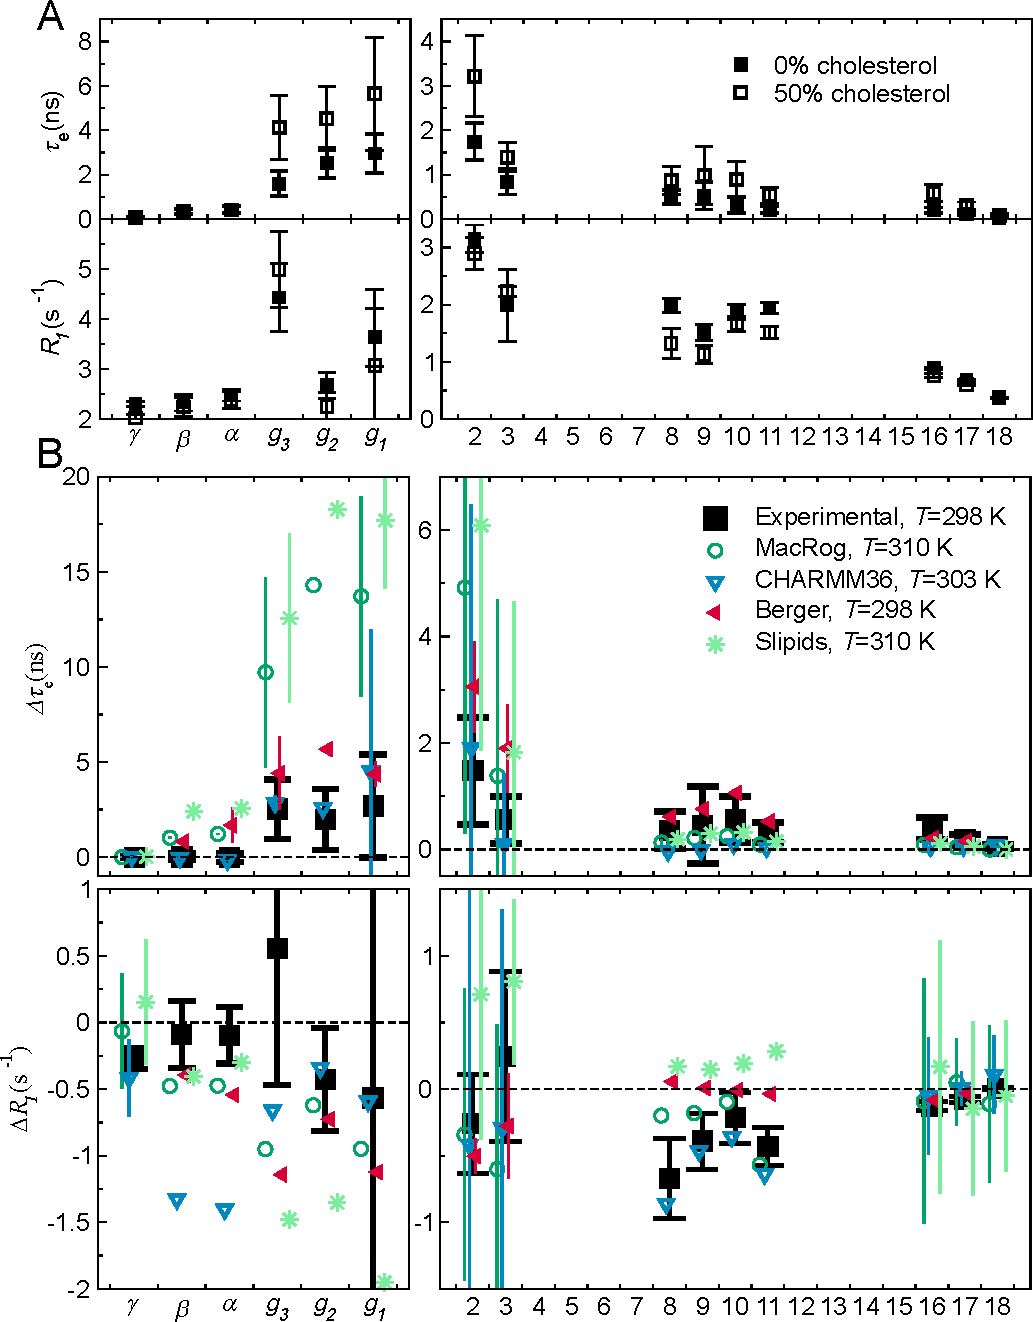
\includegraphics[scale=0.49]{cholesterol.pdf}  
\caption{The effect of bilayer cholesterol content on the effective correlation times and $R_{1}$. a) The experimental $\tau_\mathrm{e}$ (top) and $R_{1}$ (bottom) values both in pure POPC bilayer and when the bilayer contains 50\% cholesterol. The experimental data is measured at XXXK and XXX. b) The change in $\tau_\mathrm{e}$ (top) and $R_{1}$ (bottom) when bilayer composition goes from pure POPC to containing 50\% cholesterol, both experimentally and in MD simulations. Further details on the simulations are provided in Table~\ref{tab:chol}.}
\label{fig:chol}

\todo{Add A and B to fig}

\end{figure}

An assessment of the bilayer dynamics under one set of conditions does not a give complete picture of the membrane functioning. To cover wider range of the experimentally, biologically, and computationally relevant conditions, we proceed to investigate how the dynamics change when cholesterol is added to the bilayer (Fig.~\ref{fig:chol}), when the hydration level is reduced (Fig.~\ref{fig:hydration}), and when monovalent salt is added to the solution (Fig.~\ref{fig:salt}).

The addition of cholesterol causes the conformational dynamics of certain regions of POPC to slow down, whereas others stay constant. The slow-down is most evident from the experimental $\tau_\mathrm{e}$ values presented in the top panel Fig.~\ref{fig:chol}a, where a clear increase is detected for $\mathrm g_{1}$, $\mathrm g_{2}$, $\mathrm g_{3}$ and C2/C2$'$ carbons accompanied by some evidence of slower dynamics near the oleanyl double bond. The experimental $R_{1}$ rates, depicted in the lower panel of Fig.~\ref{fig:chol}a,  confirm that cholesterol addition indeed induces a change near the double bond, at the short time scale dynamics at C9 and C11 carbons. Importantly, neither experimental measure detects an effect on the headgroup $\beta$ or $\alpha$ carbons. 

All the force fields investigated in Fig.~\ref{fig:chol} qualitatively reproduce the slow down in dynamics with CHARMM36 giving the best estimate for the magnitude while Slipids clearly overestimates change, the especially at the glycerol carbons. Notably, some force fields, like Slipids, also predict a slow down for the $\alpha$ and $\beta$ carbons where no change is detected experimentally. Interestingly,  while CHARMM36 correctly gives no chance in $\tau_\mathrm{e}$, it also predicts a non-zero $\Delta R_{1}$ at $\alpha$ and $\beta$ carbons which indicates some inaccuracies in the C--H dynamics at shorter time-scales in these carbons. The tail $\Delta R_{1}$, on the other hand, seem to be well captured by CHARMM36. Along with the slow-down of dynamics, all the models show an increase in the $\vert S_{\rm{CH}}\vert$ upon addition of cholesterol at the tail region, reflecting the reduced available volume for the POPC.\todo{is this a known effect/explanation?}

The change observed here, however, is particularly sensitive to the length of the trajectory as cholesterol-induced increase in effective correlation time is likely to lead to worse convergence of the correlation function within the limited simulation time, and more drastic underestimation of $\tau_\mathrm{e}$ is expected than for simulations without cholesterol. This will, consequently, cause a tendency towards underestimation on the strength of the cholesterol-driven modulation of the effective correlation time. \todo{Should we propose that longer simulations would be good for future work? SAMULI: Only for reasonable models, like CHARMM.} 

One of the most popular models used to explain the effect of cholesterol on phopholipid bilayers is the umbrella model~\cite{huang99} where the phopholipid headgroup shields the bulky hydrophophic bodies of cholesterols from water. This leads to even distribution of cholesterol as covering single molecules is energetically less costly compared to cholesterol clusters. A recent study, using one of the most realistic MD models for cholesterol-phospholipid interactions (CHARMM36\cite{botan15}), suggested that phospholipids cover the cholesterols simply by orienting their headgroups towards the them~\cite{leeb18}. However, this effect was only detected up to 0.66 nm distance from a cholesterol molecule. Dynamically, we would expect this preferred orientation to manifest as a slow down in the headgroup C--H bonds. This is, however, not detected experimentally or with the most realistic MD models (Fig.~\ref{fig:chol}), as stipulated above, which puts the validity of the umbrella model under question. It is important to note that simulations with Berger and MacRog models do show this slow-down, possibly leading to erroneous conclusions.

To investigate the effect of hydration on the C--H bond dynamics on the PC headgroup, we first present a comparison of experimental effective correlation times obtained from the POPC (measured in full hydration) and DMPC (1,2-dimyristoyl-sn-glycero-3-phosphocholine, measured in low hydration) in Fig.~\ref{fig:hydration}a. The values are the same within the experimental accuracy, which leads to two conclusions, 1) the motions of the headgroup bonds are unaffected by the chemical differences in the tails between the two molecules and 2) the decrease of hydration level down to 13 waters per lipid does not considerably alter the correlation times for the headgroup or glycerol region. 

%As the available trajectories in low hydration are relatively short, we only investigate the effective correlation times $\gamma$ and $\beta$ carbons where the fast dynamics alleviates the risk of underestimation. 
Figure~\ref{fig:hydration}b presents effective correlation times obtained from three different MD models as function of hydration. All the force fields produce $\tau_\mathrm{e}$s that are relatively unaffected by the hydration level above 15 waters per lipid (W/L), in line with the experimental observation. When the water content is further reduced, the dynamics slows down. The effect is weakest with CHARMM36, while more  pronounced increase in $\tau_\mathrm{e}$ is observed with MacRog and Berger force fields. At these same levels of hydration, a change the lipid headgroup order parameters is also detected~\cite{botan15}, owing to the tilt of the headgroup towards the membrane plane under low hydration conditions~\cite{bechinger91}. Deuterium NMR relaxation time ($T_{1}$) measurements from DOPC bilayers~\cite{ulrich94} have revealed a slow-down of the headgroup conformational dynamics below $\approx$10 W/L, which was attributed to the reduction in available volume for the tilted headgroup. This slow-down is in qualitatively in line with the increased $\tau_{\rm{e}}$ observed here from the MD models. 


\todo{SAMULI: Maybe we could have a quantitative discussion about how much dehydration slows down the dynamics and how this could affect, e.g., to membrane fusion.} 

\todo{SAMULI: It would be interesting to compare the acyl chains with dehydration to the ones with cholesterol.}
  
In the tail region dehydration also causes a consistent decrease in $\tau_{\rm{e}}$ when using the Berger and MacRog models (data not shown). This change is accompanied by an increase in the absolute value of the tail order parameters, which may serve as the early indicators of structural transition in the bilayer upon dehydration in the MD models.  Experimentally, the gel-to-liquid crystalline phase transition occurs around 3~W/L at room temperature~\cite{lynch89}.\todo{validity of "structural transition" -statement}

The observed general slow down is of significance when studying not only single bilayers under low hydration but also intermembrane interactions, such as fusion, which naturally lead to dehydrated conditions as the lipid assemblies approach. Slower dynamics imply that longer simulation times are needed for equilibration, for reliably quantifying the properties of the bilayer, and for observing any dynamic events like the lipid tail flips from one membrane to another in case of the fusion~\cite{best citation here}. Same applies in simulations performed in increasing concentrations of cholesterol, as the slow down of dynamics and the increase of tail order parameters observed therein are analogous to those occurring upon dehydration. \todo{really not the smoothest text}

\begin{figure}[ht!]
\centering
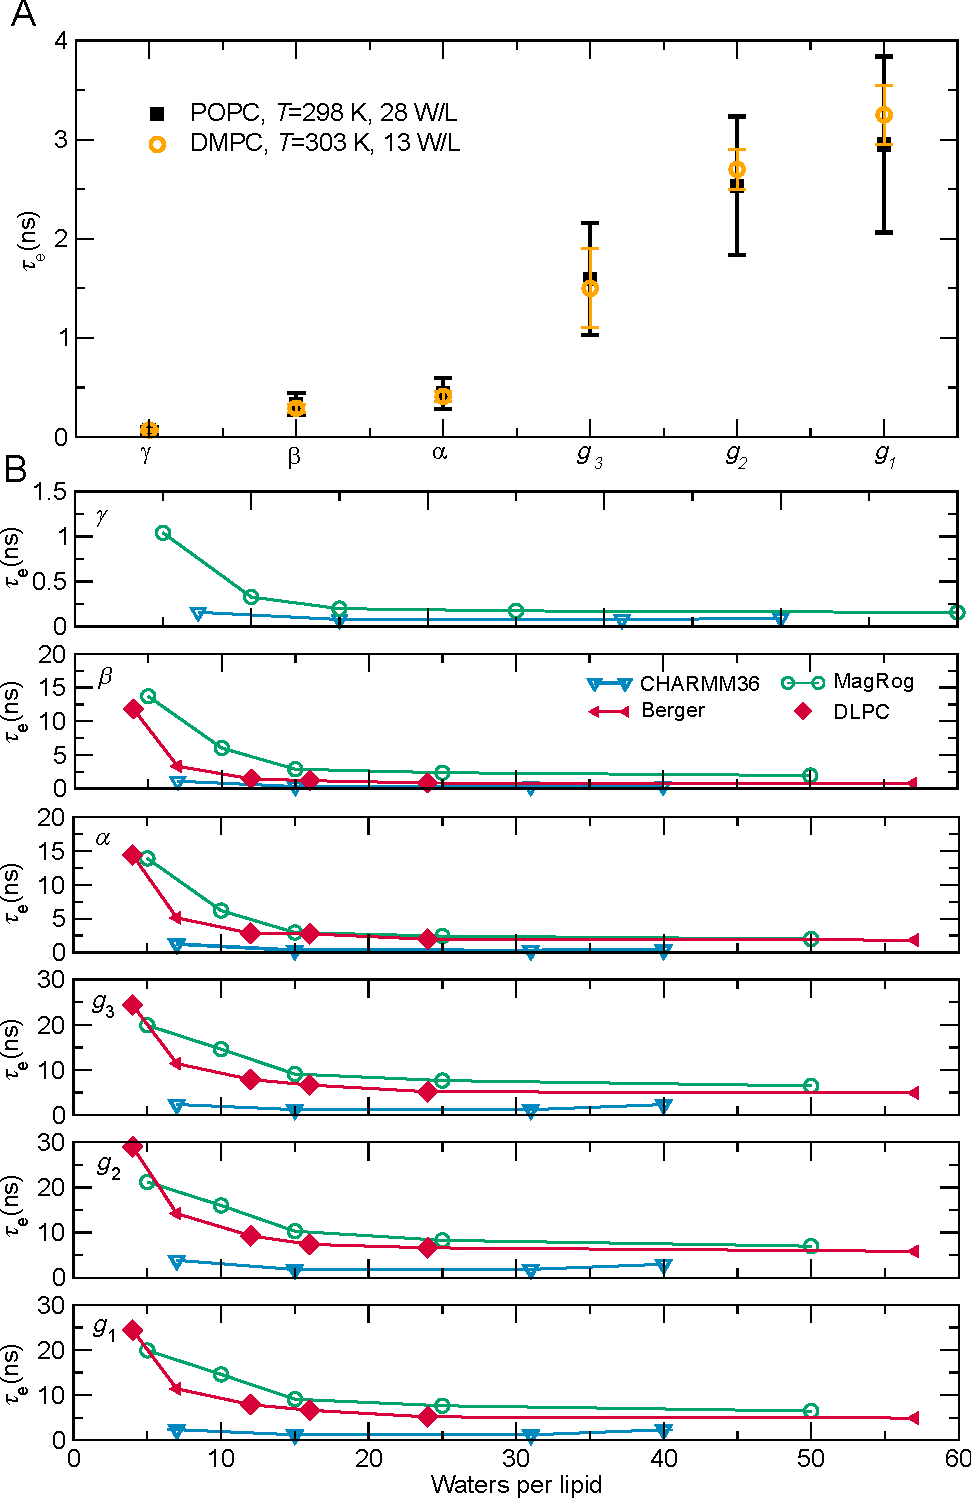
\includegraphics[scale=0.51]{hydration.pdf} 

\caption{The effect of hydration on the effective correlation times. a) Comparison of experimental effective correlation times from DMPC in low hydration (13 W/L) and POPC in full hydration (28 W/L). The DMPC data is obtained from Ref.~\citenum{pham15} whereas the POPC data is as in Figures~\ref{fig:teff_R1}. Neither the different chemistry of the lipid tails, nor the hydration level has an effect within the experimental accuracy. b) The response of effective correlation times to changing hydration level from three MD models. The error bars give the minimum and maximum value observed at each carbon while the symbol denotes the average. The change in the effective correlation time, $\Delta \tau_\mathrm{e}$, is quantified with respect to the salt-free state. Details on the simulations are given in 
Table~\ref{tab:hydr}. Note that three of the data points for the Berger model are from 1,2-didodecanoyl-sn-glycero-3-phosphocholine (DLPC) bilayers (diamonds). }
\label{fig:hydration}

\todo{how to refer to full hydration POPC data}
\end{figure}


Finally, we study the response of the MD model dynamics to increasing amounts of monovalent salt. Experimentally, the modulation of $\alpha$ and $\beta$ carbon order parameters upon increasing ion concentration have been used to quantify ion binding to lipid bilayers (the molecular electrometer~\cite{seeling87,catte16}). The order parameters are constant for POPC bilayers under NaCl addition in experiments, indicating negligible ion binding. Based on this, we anticipate the effective correlation times also to be unaffected by monovalent salt, however, to our knowledge no experimental measurements have been conducted to quantify this.

The molecular electrometer has been used to show that most molecular dynamics force fields overestimate the binding of monovalent ions to PC bilayers~\cite{catte16}: In the simulations the modulation of the $\alpha$ and $\beta$ carbon order parameters by increasing NaCl concentration was overestimated compared to the experiments, and accompanied by accumulation of ions at the bilayer surface. In Fig.~\ref{fig:salt} we compare three force fields, one that is known to exhibit pronounced overbinding~\cite{catte16} (MacRog) and two producing more realistic binding affinity (Slipids and CHARMM36). The lateral distribution of Na$^{+}$ ions near the bilayer is quantified in Fig.~\ref{fig:salt}a whereas Fig.~\ref{fig:salt}b shows the chance in $\tau_{\rm{e}}$ for increasing salt concentration. Ion accumulation results in a slow down in the effective correlation time that is somewhat proportional to the strength of ion binding. Correlation times extracted from the CHARMM36 model vary only a little (low ion binding) when ion concentration is increased, whereas a slightly more pronounced change is observed with Slipids, and MacRog exhibits a clear slow-down (significant ion binding). This indicates that, similarly to the order parameters, $\tau_{\rm{e}}$ may be useful in investigating the ion binding affinity of lipid bilayers and experimental work exploring this avenue would be interesting.   

\todo{validity of statement regarding Slipids}

\begin{figure}[ht!]
\centering
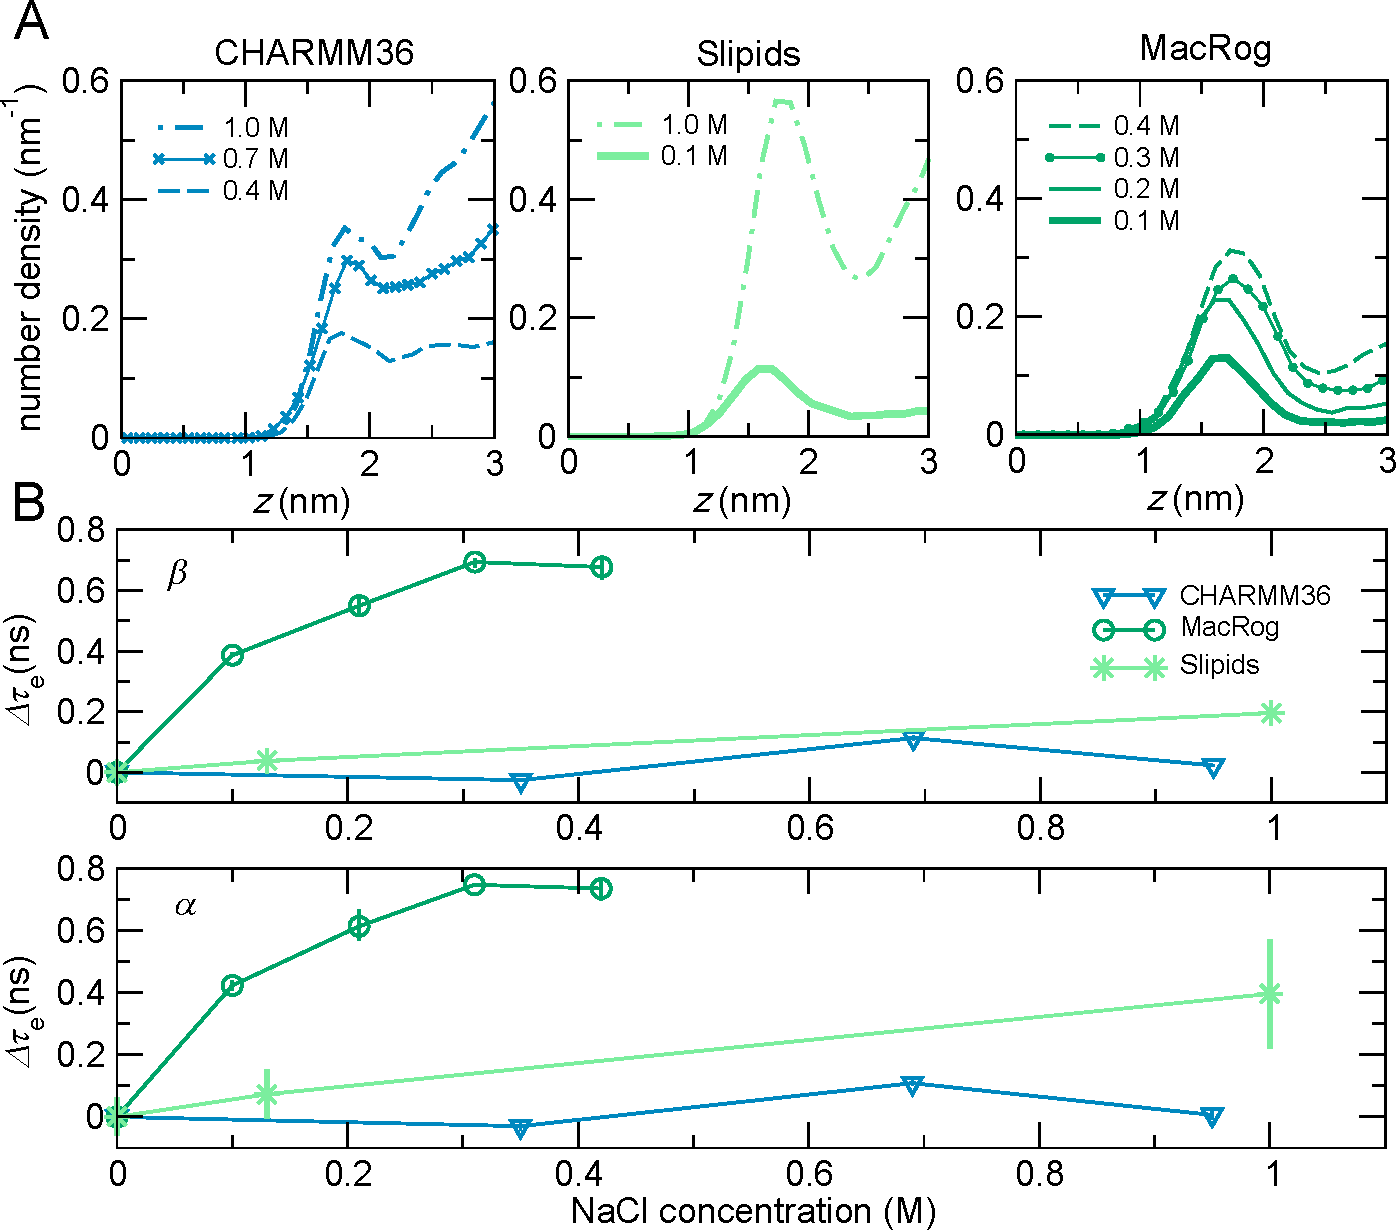
\includegraphics[scale=0.36]{salt.pdf} 
\caption{The impact of increasing ionic strength on effective correlation times. a) The density distribution (average over both leaflets) of Na$^{+}$ ions as function of distance $z$ from the bilayer center. The plots for each force field are presented from left to right in the order of increasing ion accumulation. b) Effective correlation times for $\alpha$ and $\beta$ C--H bonds in growing NaCl concentration from CHARMM36, Slipids, MacRog POPC simulations. Details on the simulation data are provided in Table~\ref{tab:salt}.}
\label{fig:salt}
\end{figure}




\section{Conclusions}


Here, we have investigated the dynamics of phosphatidylcholine molecular dynamics models using publicly available MD trajectories. The MD models are able to qualitatively capture the correlation time profile of POPC---the slow glycerol backbone and the faster dynamics of the headgroup and tail regions---but most are prone to too slow dynamics of the glycerol C--H bonds.  In general, the these force fields reproduce the experimentally detected $R_{1}$ values adequately, indicating that processes at time scales $\sim$1 ns are represented but problems arise at longer time-scales. While none of the force fields is able to reproduce all the experimental values, the CHARMM36 POPC model performs well when compared to the effective correlation times, while the Slipids and Lipid14 force field provide realistic $R_{1}$ in the PC headgroup and glycerol regions. However, since none of the current MD models reproduce the experimental order parameters, these timescales depict a sampling of a conformational space that does not fully represent the underlying reality.


In addition to the bilayers under standard conditions, we also explored how the dynamics react to the addition of cholesterol, salt, and to the reduction of hydration level. When cholesterol is mixed into the POPC bilayer, the conformational dynamics of the tails and the glycerol regions slows down. Again, the MD models are able to qualitatively capture this, but some also predict an increase in the correlation times for the headgroup carbons, possibly leading to erroneous conclusions. In increasing salt concentration a behaviour reminiscent of the molecular electrometer was observed: Amount of ion binding to the bilayer correlated with the magnitude of slowdown in the correlation times. This could open up the possibility of using effective correlation times in quantifying the ion binding to lipid bilayers. When reducing the water content, the MD models exhibited somewhat constant correlation times down to $\sim$15 waters per lipid in agreement with experimental data. After this, a slow down was observed.\todo{hydration needs some kind of statement of significance.}

By gathering a set of experimental information on the phosphatidylcholine dynamics and underlining some of the typical features of the MD models, this study sets a foundation and a potential roadmap for further improvement of the current force fields. While work is still needed in capturing even the correct order parameters, the dynamics is equally essential part of developing MD into a true computational microscope; after all, it is possible to obtain the correct order parameters just by freezing the system into a set of selected conformations.\todo{not very smoothly put, help!}  

Finally, this work demonstrates the power of open data in creating new knowledge out of existing trajectories at a reduced computational and labor cost. Although no new simulations were performed for the purpose of this work, we were able to conduct a comprehensive study on the dynamics of MD models under several conditions. An interesting extension would be exploring other lipid headgroups individually as well as performing a comparison of MD model dynamics between headgroup types, as the available simulation data goes well beyond simulations of lipids with the phosphocholine headgroup. If the data are well indexed and documented, this process could be easily automated and has the potential to facilitate faster progress, eg., in the development of lipid (and other) MD models. Naturally, such database would provide a fruitful platform to other machine learning applications as well. 


\acknowledgement
  This material is based upon work supported by XXX under Grant No. XXX. The project is/isn't part of the NMRlipids open collaboration (nmrlipids.blogspot.com)

\bibliography{lipids,ff,simu,pdb,journals}

\begin{tocentry}
 % \includegraphics[width=77mm]{abstract_figure}
 TOC here if needed
\end{tocentry}

\end{document}
